\documentclass[conference]{./../../IEEE/IEEEtran}

\usepackage[dvips]{graphicx}
\usepackage[T1]{fontenc}
\usepackage{amsmath}
\usepackage{amsfonts}
\usepackage{balance}
\usepackage{algorithm}
\usepackage{algorithm,acronym}
\usepackage{subeqnarray,cite,mathtools}

\graphicspath{{./../Figures/}}

\input{./../../Common/acronyms}
\input{./../../Common/shortcuts}

\begin{document}

\title{Implementation of MU-MIMO Schedulers on SoC}
%\vspace{-22ex}

\author{\begin{tabular}{cc}
\multicolumn{2}{c}{Ganesh Venkatraman, Janne Janhunen, Markku Juntti}\\
Centre for Wireless Communications (CWC), & Department of Communication Engineering (DCE), \\
\multicolumn{2}{c}{University of Oulu, Oulu, FI - 900 14}\\
\end{tabular}}

\maketitle

\acused{MIMO}

\begin{abstract}
	
To avail the complete advantages of a multi-antenna system, \ac{MU-MIMO} technique is performed by multiplexing different user data streams spatially over a time-frequency resource. However, serving tens of users in \ac{MIMO} systems increases the scheduler complexity significantly. In this paper, we study the computational complexity of different state-of-the-art \ac{MU-MIMO} scheduling algorithms and evaluate the number of users we are able to serve with current technology taking into account the given real-time requirements. To provide a fair comparison, we first analyze the achievable sum rate performance of various scheduling algorithms using MATLAB simulator. We then implement the scheduling algorithms on real hardware, i.e., Xilinx ZYNQ-7000 series multi-core ARM-FPGA \ac{SoC} to show how current systems can take advantage of \ac{MU-MIMO} techniques.
\end{abstract}

\acresetall
\acused{MIMO}
\section{Introduction}
The current wireless standards are moving towards the packet switched networks to improve the system performance and flexibility as compared to the circuit switched networks. The radio access technologies aim at achieving higher throughput and better system performance but still targeting to low energy budget. The use of multi-antenna transmission is \textit{de-facto} in all upcoming standards, favoring the spatial multiplexing of user data by applying transmit precoders for \ac{MU-MIMO} transmission. In order to achieve the best possible benefit of the \ac{MU-MIMO} transmission, the multiplexed users should have channel vectors as linearly independent as possible. The linear independency condition arises by designing linear precoder at the transmitter to decouple the user streams at the receiver end. The selection of users with such a constraint is carried out by the schedulers to utilize the wireless system resources efficiently.

The scheduling algorithms based on the sum rate maximization objective for \ac{MU-MIMO} are discussed thoroughly in the literature. The search based on successive projections (SP) scheme for single-antenna receiver is discussed in \cite{sus2006zfbf} and the extension for multi-antenna receivers are provided in \cite{Tolli-etal-2005}. In \cite{Tolli-etal-2005}, the users are selected by choosing the user with the maximum gain on to the orthogonal subspace. The orthogonal subspace is evaluated as the null space of the stacked channel vectors of the already chosen users over earlier iterations. Similar algorithms addressing a lower computational complexity are proposed in \cite{shen2006low} and \cite{youtuan2007improved}. User selection based on the volume maximization metric are discussed in \cite{jin2010novel}. The performance of the volume based selection is identical to the SP or block diagonal (BD) scheme, since both schemes use Gram-Schmidt (GS) procedure.

In this paper, we study the computational complexity of different state-of-the-art \ac{MU-MIMO} scheduling algorithms and evaluate the number of users we are able to serve in the system. Current work excludes precoding implementation, but in future, we will include a two-step scheduling-precoding design approach, where the scheduler identifies a subset of users in the first step and then precoders are designed for the chosen subset in the second step. To enable a fair comparison, we first analyze the achievable sum rate performance of the different algorithms and then we discuss the implementation of the scheduling schemes on real hardware, i.e., Xilinx Zynq 7000 ZC702 evaluation platform, to show how current systems can take advantage of \ac{MU-MIMO} techniques. This work is a continuation to our previous implementation studies \cite{Janhunen-etal-11, Hanninen-etal-2014, Shahabuddin-etal-2014} aiming to find low-power but high performance solutions for the advanced long term evolution (LTE-A) transceivers.

Even though the achievable sum rate 

The paper is organized as follows. Single-cell downlink system model is described in Section \ref{sec:system_model}. Section \ref{sec:perf_scheduling} presents performance comparison between selected scheduler schemes using link level simulations. In Section \ref{sec:implementation}, implementations results of different scheduling algorithms mapped on Xilinx ZYNQ ZC702 \ac{SoC} are presented. Finally, Section \ref{sec:conclusion} summarizes the conclusions and future work.

\section{System Model}
\label{sec:system_model}
We consider a single-cell downlink \ac{MU-MIMO} transmission with \eqn{N_T} transmit antennas and \eqn{K} \ac{N_R} antenna users. The transmission is carried out by multiplexing user signals in the spatial dimensions. Since the users are transmitted on the same time-frequency resource, the received signal \eqn{y_k} of the user \eqn{k} with interference is given by
\begin{equation}
y_k = \mvec{h}{k} \mvec{x}{k} + \sum_{i \in \mathcal{S} \backslash \{k\}} \mvec{h}{k} \mvec{x}{i} + n_k,
\end{equation}
where \eqn{\mathcal{S}} is the set having the indices of the multiplexed users at a given scheduling instant. The transmitted signal for user \eqn{k} is denoted by \eqn{\mvec{x}{k} = \mvec{m}{k} d_k}, where \eqn{\mvec{m}{k} \in \mathbb{C}^{N_T \times 1}} is the transmit precoder and \eqn{d_k} denotes the data meant for user \eqn{k} with unit energy as represented by \eqn{\mathbf{E}[|d_k|^2] = 1}. The channel between the user \eqn{k} to the cell is given by \eqn{\mvec{h}{k} \in \mathbb{C}^{1 \times N_T}} and \eqn{n_k} is the complex Gaussian noise added at the receiver, drawn from \eqn{\sim \mc{CN}(0,N_0)}, zero mean and variance \eqn{N_0}.

Let \eqn{\mathcal{U}} be the set consisting of all users in the system. The objective of the scheduler is to select users with the channel vectors as linearly independent as possible for the set \eqn{\set{\mathcal{S} \subset \mathcal{U}}} at each scheduling instant to maximize a sum rate maximization (SRM) objective. Selecting a subset \eqn{\mathcal{S}} from the set \eqn{\mathcal{U}} is a combinatorial problem in general requiring an exhaustive search of \eqn{O(K^{N_T})} complexity.

A scheduler based on a successive projection (SP) selects the user by projecting the channel vectors on to the null space of the existing user channel vectors as in \cite{sus2006zfbf,antti_user_selection}. Initially, the user with higher channel gain from the set \eqn{\mathcal{U}} is selected for the transmission set \eqn{\mathcal{S}}. Then, the remaining users are selected from \eqn{\mathcal{U} \backslash \mathcal{S}} by projecting the channel vector on to the null space of the user channel vectors in \eqn{\mathcal{S}}. The selection metric of a user is given as
\begin{subeqnarray}
\mbf{H} &=& \left [ \mvec{h}{\mathcal{S}(1)}^T,\dotsc,\mvec{h}{\mathcal{S}(|\mathcal{S}|)}^T \right ] \slabel{eqn-1.0} \\
\mbf{N}(\mathcal{S}) &=& \mbf{I}_{N_T} - \mbf{H} \left (\mbf{H}^H \mbf{H} \right )^{-1} \mbf{H}^H \slabel{eqn-1.1} \\
m_i &=& \| \mbf{N}(\mathcal{S}) \, \mvec{h}{i}^T \|^2, \; \forall \, i \, \in \mathcal{U} \backslash \mathcal{S} \slabel{eqn-1.2}\\
\bar{u} &=& \underset{i}{\arg \max} \; \; m_i, \quad \mathcal{S} = \mathcal{S} \cup \set{\bar{u}},
\label{eqn-1}
\end{subeqnarray}
where \textbf{N} denotes the null space matrix and $\mbf{I}_{N_T}$ is the identity matrix of size $N_T$. The above metrics are evaluated at each iteration to identify a user until the condition $|\mc{S}| = N_T$ is satisfied.

We also consider a product of independent projection displacements (PIPD) algorithm requiring minimal computational complexity compared to the successive projection scheduling scheme. The complexity involved in selecting the first user remains the same, since the user with the highest channel norm is considered for the set \eqn{\mc{S}} in both schemes. The complexity of selecting the remaining users are significantly reduced by the PIPD scheduling scheme using the product of independent vector projection displacements metric. More detailed description of the algorithm is presented in \cite{Venkatraman-etal-14}.

Figure \ref{kuva:scheduler_block_diag} illustrate the operations involved in the metric calculations for greedy, SP and PIPD scheduling schemes. The blocks mentioned separately for the PIPD and the SP schemes are executed based on the selected algorithm. Greedy algorithm requires only the norm calculation of the virtual channel vectors with which the sorting operation can be used to find the leading $N_T$ users for the set $\mathcal{S}$. In the case of the SP selection scheme, the users are identified by projecting the corresponding channel vectors on to the null space of the existing users channel vectors and selecting the one with the maximum projection gain. In order to evaluate the null space, a matrix inversion is required demanding significant complexity as compared to the matrix multiplications approach used in the PIPD algorithm in Figure \ref{kuva:scheduler_block_diag}.

For example in computer simulation, the complexity involved in evaluating the null space of a matrix of $4 \times 3$ requires $44 \, 972$ cycles, which includes a $3 \times 3$ matrix inversion requiring $35 \, 539$ cycles, providing a major share in the complexity of the metric expression for the SP scheme. On the other hand, the PIPD scheme requires only the inner product evaluations of a $4 \times 1$ vectors requiring $1 \, 693$ cycles and the norm of a $4 \times 1$ vector requires $144$ cycles, providing significant complexity reductions. In Figure \ref{kuva:scheduler_block_diag}, the PIPD metric $P_i$ requires significantly less computations as compared to the SP null space metric $\mathbf{N}(\mc{S})$ calculation in order to obtain the projection metric to identify a dominant user at each iteration.

%%%figure code
\begin{figure}[htb]
%\begin{minipage}[b] {1.0\linewidth}
\centering
%\vspace{-3ex}
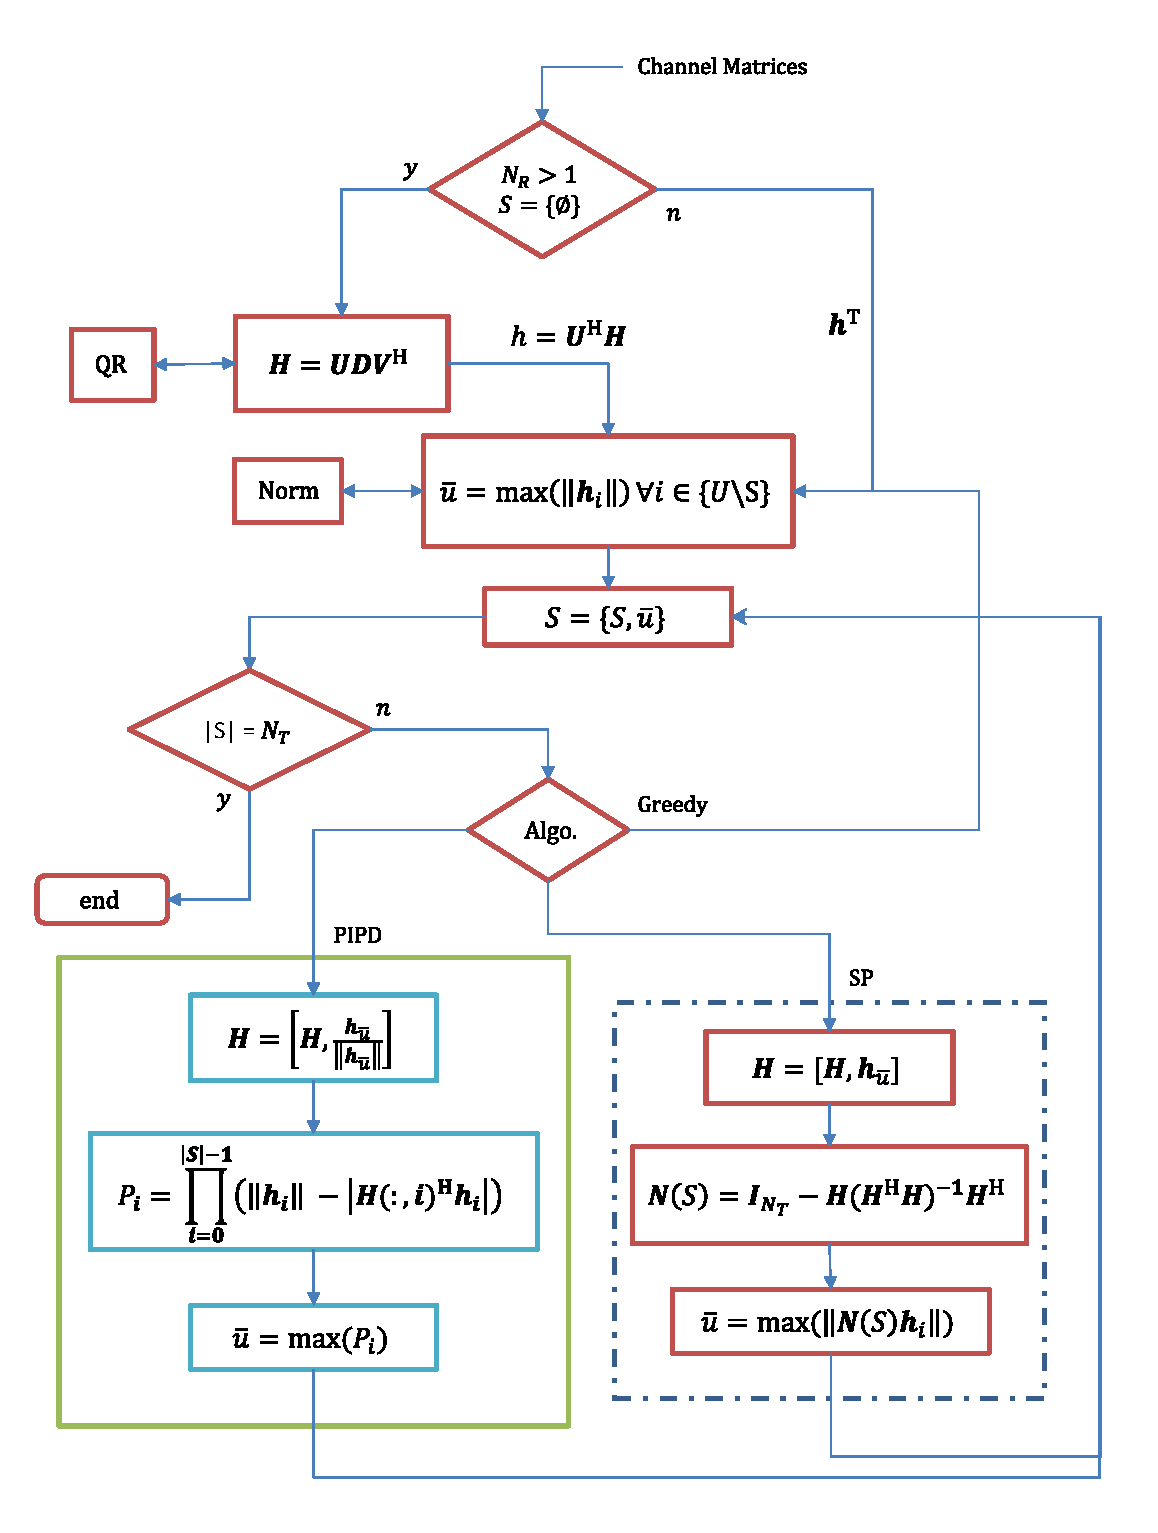
\includegraphics[width=9.0cm, angle=0]{scheduler_figure_updated2.eps}
%\vspace{-3ex}
\caption{System model.}
\label{kuva:scheduler_block_diag}
%\end{minipage}
\end{figure}

\section{MU-MIMO Scheduling}
\label{sec:perf_scheduling}
\subsection{MU-MIMO Selection}

The practical scenarios for the MU-MIMO technique to enhance the throughput in the LTE-A system are addressed in the existing literature to a large extent. The transmission user set $\mathcal{S}$ is usually identified from the pool of users consisting the users of the first transmission attempt. Once a user is identified for the set $\mathcal{S}$, the remaining users are usually identified from the user set with the retransmission attempts instead of the initial transmission. Since the primary user is selected initially, the transmission is prioritized for the primary transmission user.

\subsection{Scheduling Resolution}
The scheduling is performed over the scheduling blocks (SBs) and the resolution of a SB significantly affects the performance of the overall throughput. For instance, if the SB resolution is equal to the physical resource block (PRB), the scheduling complexity increases linearly with the number of SBs and the throughput performance depends on the number of users in the system. Thus, if the SB equals one PRB and the number of users is large, the performance will be improved by utilizing the multi-user (MU) diversity with the help of a proper scheduling scheme. However, if the users are few in number, the performance degradation is quite significant due to the smaller coding length and lack of channel variations over the smaller SB to extract the channel diversity in the form of coding gain. In case of larger SB size with grouped PRBs, the scheduling complexity will be reduced significantly but the network throughput will also reduce noticeably, unless the channel fading over frequency domain is flat or nearly flat. In this scenario, the users with the transmission in such scheduling will attain higher throughput due to the longer coding length which needs to be quantified only at the system level.

\subsection{Scheduling Performance}

Fig. \ref{kuva:performance_plot} compares the sum rate performance of four different scheduling schemes with $\textrm{N}_T = 4$ and $K = 50$ users. The sum rate performance of the PIPD scheme performs close to the SP scheme. The figure also shows a larger gap (approximately 10 bit/sec/Hz) between Norm/Greedy scheme which selects users based on the channel norm only and PIPD scheduling scheme. Round Robin scheme performs worst as expected. The performance of the PIPD scheme degrades as the size of the channel matrix increases from $4 \times 1$ to $4 \times 2$ owing to the approximations performed in the algorithm instead of computing matrix inversion.

%%%figure code
\begin{figure}
\centering
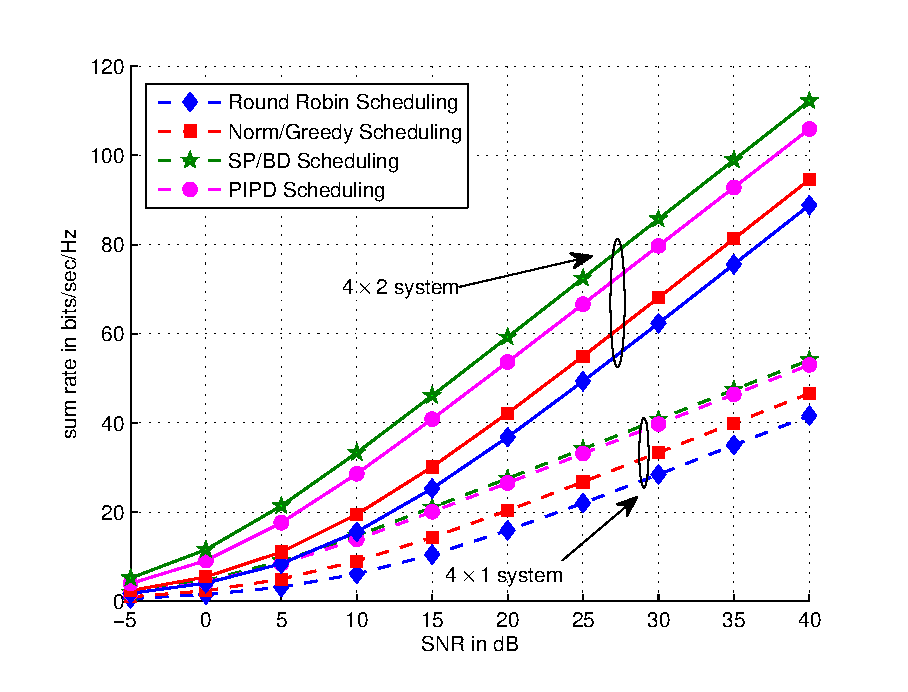
\includegraphics[width=9.0cm, angle=0]{performance_plots.eps}
\caption{Performance comparison of scheduler algorithms.}
\label{kuva:performance_plot}
\end{figure}

\subsection{Complexity Analysis}
In this section, we discuss the complexities involved in the scheduling procedure for various system configurations which
are used in the standard system deployment. Before implementing scheduler on a real processing platform we did a careful evaluation of schedulers on MATLAB and C-based simulators. MATLAB simulator provides for a good performance simulation environment for comparing scheduler algorithm, whereas the C-simulator is used to identify processing complexities. In C-simulator we applied BLAS (Basic Linear Algebra Subprograms) and LAPACK (Linear Algebra PACKage) libraries. The libraries include optimized functions for linear algebra and vector math providing for example optimized SVD and matrix multiplications. Programming the simulator using libraries enables a fair comparison between scheduler algorithms enabling the best implementation of complex functions. Simulator results are run on Intel's core.

Table \ref{table:compexity_comparison} compares the complexity involved in the scheduling procedure for different number of users and the scheduling blocks in the system. The table uses GPRB which represents the number of PRBs grouped to form a scheduling block, which in this case is set to be $5$ PRBs. The scheduling block is the resource entity for which the scheduler decides the transmitting user set $\mathcal{S}$. The NPRB denotes the number of PRBs present in the system and the performance of all the schemes discussed earlier are listed for various configurations in Table \ref{table:compexity_comparison}. In the complexity analysis, we consider $\textrm{N}_R$ as the number of receive antennas at each user in the system. As $\textrm{N}_R \geq 2$, singular value decomposition (SVD) is used to decompose the channel in order to treat the spatial streams as a virtual users in the scheduling procedure. In case of a $4 \times 2$ system, the total number of cycles required to decompose the channel matrix using SVD for $20$ and $50$ users are $5 \, 022 \, 947$ and $12 \, 492 \, 227$ cycles, respectively. The matrix multiplication of $4 \times 4$ null space matrix $\textbf{N}(\mathcal{S})$ in Figure \ref{kuva:performance_plot} with a vector of $4 \times 1$ $h_i$ contributes $599$ cycles. This multiplication happens in the PIPD and the SP scheme demands for more computational power compared to the greedy algorithm which doesn't have the operation.

%The cycle contribution of $120$ attributed to the matrix multiplications performed in the SP and the PIPD schemes alone for

%%Table of Processor FUs
\begin{table}[ht!]\caption{Complexity of the Scheduling Schemes} \vspace{-3ex}\begin{center} \small
\begin{tabular}{l r r r r}
$\textit{N}_T \times \textit{N}_T$ & \textit{K} & Successive     & PIPD          & Greedy \\
                                   &            & Projections    & with mem      &        \\ \hline
$4 \times 1$                       & 20         & 936\,907       & 240\,164      & 77\,618  \\
$4 \times 1$                       & 50         & 1\,764\,598    & 579\,462      & 184\,296 	\\
$4 \times 2$                       & 20         & 1\,418\,373	 & 415\,329      & 109\,501   \\
$4 \times 2$                       & 50         & 2\,986\,142    & 1\,017\,318   & 264\,240 	\\ \hline
\end{tabular} \label{table:compexity_comparison}\end{center}\end{table}

The sum rate performance of the PIPD scheme performs close to the SP scheme with the complexity
comparable to the max-norm scheduling scheme which selects users based on the channel norm only.


\section{Implementation results}
\label{sec:implementation}
In this section, we will describe the scheduler implementation on Texas Instruments' multicore DSP. The results will show the number of served users with a state-of-the-art DSP platform reaching real-time processing requirements. We expect SVD to cause latency problems and possibly requiring hardware acceleration to meet the strict real-time requirements. We will analyze the performance of the SVD and the metric evaluations with the algorithms discussed earlier to identify the possible parameters values in order to meet the real-time requirement of $1$ ms scheduling periodicity used in the various upcoming standards.


\section{Conclusions and Future Work}
\label{sec:conclusion}
We studied the computational complexity of different state-of-the-art MU-MIMO scheduling algorithms. We showed that most of the computational complexity in MU-MIMO scheme is caused by the SVD but also matrix multiplications cause significant computational complexity. Already computer simulations indicate that SVD may require hardware acceleration and in future we will study the possibility to accelerate implementation with a field programmable gate array (FPGA).

\section*{Acknowledgment}
This research was done in BaSE (Baseband and System Technologies for Wireless Evolution) project supported by the Finnish Funding Agency for Technology and Innovation (Tekes), Nokia Solutions and Networks, Broadcom, Xilinx and Elektrobit.

\bibliographystyle{./../../IEEE/IEEEtran}
\bibliography{./../../IEEE/IEEEabrv,./../biblio/bibliography}
%\bibliography{./../biblio/bibliography}

\end{document}


